% This file was created by matlab2tikz.
%
\documentclass[tikz]{standalone}
\usepackage[T1]{fontenc}
\usepackage[utf8]{inputenc}
\usepackage{pgfplots}
\usepackage{grffile}
\pgfplotsset{compat=newest}
\usetikzlibrary{plotmarks}
\usetikzlibrary{arrows.meta}
\usepgfplotslibrary{patchplots}
\usepackage{amsmath}

\newlength\figureHeight \setlength{\figureHeight}{6cm}
\newlength\figureWidth \setlength{\figureWidth}{10cm}
\begin{document}
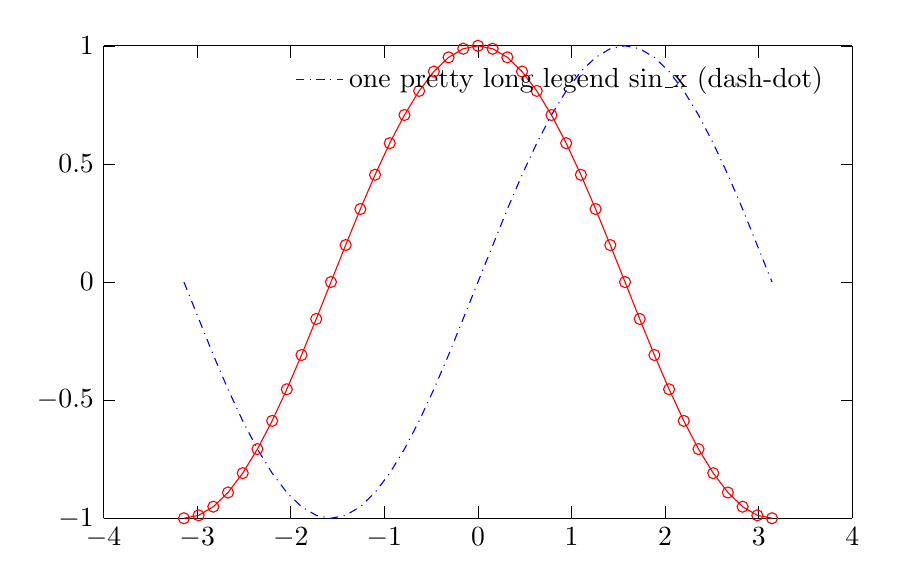
\begin{tikzpicture}

\begin{axis}[%
width=0.951\figureWidth,
height=\figureHeight,
at={(0\figureWidth,0\figureHeight)},
scale only axis,
separate axis lines,
every outer x axis line/.append style={black},
every x tick label/.append style={font=\color{black}},
every x tick/.append style={black},
xmin=  -4,
xmax=   4,
every outer y axis line/.append style={black},
every y tick label/.append style={font=\color{black}},
every y tick/.append style={black},
ymin=  -1,
ymax=   1,
axis background/.style={fill=white},
legend style={legend cell align=left, align=left, fill=none, draw=none}
]
\addplot [color=red, mark=o, mark options={solid, red}, forget plot]
  table[row sep=crcr]{%
-3.14159	  -1\\
-2.98451	-0.987688\\
-2.82743	-0.951057\\
-2.67035	-0.891007\\
-2.51327	-0.809017\\
-2.35619	-0.707107\\
-2.19911	-0.587785\\
-2.04204	-0.45399\\
-1.88496	-0.309017\\
-1.72788	-0.156434\\
-1.5708	   0\\
-1.41372	0.156434\\
-1.25664	0.309017\\
-1.09956	0.45399\\
-0.942478	0.587785\\
-0.785398	0.707107\\
-0.628319	0.809017\\
-0.471239	0.891007\\
-0.314159	0.951057\\
-0.15708	0.987688\\
   0	   1\\
0.15708	0.987688\\
0.314159	0.951057\\
0.471239	0.891007\\
0.628319	0.809017\\
0.785398	0.707107\\
0.942478	0.587785\\
1.09956	0.45399\\
1.25664	0.309017\\
1.41372	0.156434\\
1.5708	   0\\
1.72788	-0.156434\\
1.88496	-0.309017\\
2.04204	-0.45399\\
2.19911	-0.587785\\
2.35619	-0.707107\\
2.51327	-0.809017\\
2.67035	-0.891007\\
2.82743	-0.951057\\
2.98451	-0.987688\\
3.14159	  -1\\
};
\addplot [color=blue, dashdotted]
  table[row sep=crcr]{%
-3.14159	  -0\\
-2.82743	-0.309017\\
-2.67035	-0.45399\\
-2.51327	-0.587785\\
-2.35619	-0.707107\\
-2.19911	-0.809017\\
-2.04204	-0.891007\\
-1.88496	-0.951057\\
-1.72788	-0.987688\\
-1.5708	  -1\\
-1.41372	-0.987688\\
-1.25664	-0.951057\\
-1.09956	-0.891007\\
-0.942478	-0.809017\\
-0.785398	-0.707107\\
-0.628319	-0.587785\\
-0.471239	-0.45399\\
-0.314159	-0.309017\\
   0	   0\\
0.314159	0.309017\\
0.471239	0.45399\\
0.628319	0.587785\\
0.785398	0.707107\\
0.942478	0.809017\\
1.09956	0.891007\\
1.25664	0.951057\\
1.41372	0.987688\\
1.5708	   1\\
1.72788	0.987688\\
1.88496	0.951057\\
2.04204	0.891007\\
2.19911	0.809017\\
2.35619	0.707107\\
2.51327	0.587785\\
2.67035	0.45399\\
2.82743	0.309017\\
3.14159	   0\\
};
\addlegendentry{one pretty long legend sin\_x (dash-dot)}

\end{axis}
\end{tikzpicture}%
\end{document}